
%(BEGIN_QUESTION)
% Copyright 2007, Tony R. Kuphaldt, released under the Creative Commons Attribution License (v 1.0)
% This means you may do almost anything with this work of mine, so long as you give me proper credit

Some flow-measuring instruments are of the {\it insertion} type, such as this Annubar unit.  Here, the Annubar tube passes through the middle of a ball valve, with a compression-style ferrule and nut used to seal process fluid from leaking out of the assembly:

$$\includegraphics[width=15.5cm]{i00047x01.eps}$$

Describe how an insertion-type flowmeter such as this may be removed from an operating pipe, and then re-installed, {\it all without interrupting the flow of process fluid through the pipe}.


\underbar{file i00047}
%(END_QUESTION)





%(BEGIN_ANSWER)

To remove:

\begin{itemize}
\item{} Loosen the gland nut until the insertion body can move up and down
\item{} Withdraw the Annubar unit from the pipe until the end clears the ball isolation valve
\item{} Shut the ball valve
\item{} Remove the gland nut entirely
\item{} Pull the Annubar completely out of the pipe
\end{itemize}

\vskip 10pt

To re-install, reverse all steps!

%(END_ANSWER)





%(BEGIN_NOTES)


%INDEX% Measurement, flow: servicing an insertion-type flowmeter

%(END_NOTES)


